\renewcommand*{\arraystretch}{1.1}

\noindent\begin{tabularx}{17cm}{|p{1.95cm}|X|}
	\hline
	workload    & Interactive \\ \hline
%
	query       & 10 \\ \hline
%
	title       & Friend recommendation \\ \hline
%
    pattern     & \hfill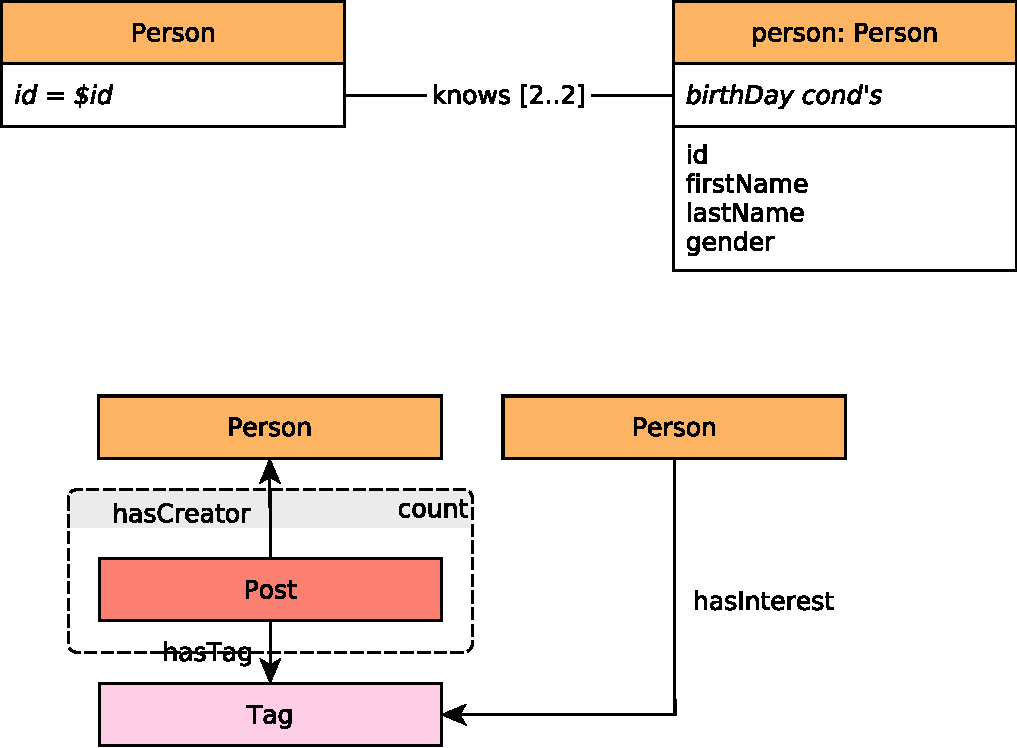
\includegraphics[scale=\patternscale,margin=0cm .2cm]{patterns/interactive10}\hfill\vadjust{} \\ \hline
%
	description & Given a start Person, find that Person's friends of friends (excluding
start Person, and immediate friends), who were born on or after the 21st
of a given month (in any year) and before the 22nd of the following
month. Calculate the similarity between each of these Persons and start
Person, where similarity for any Person is defined as follows:

\begin{itemize}
\tightlist
\item
  common = number of Posts created by that Person, such that the Post
  has a Tag that start Person is Interested in
\item
  uncommon = number of Posts created by that Person, such that the Post
  has no Tag that start Person is Interested in
\item
  similarity = common - uncommon
\end{itemize}
 \\ \hline
	
%
	parameters  &
	\vspace{1.1ex}{\begin{tabularx}{14.2cm}{|c|M|m{2cm}|Y|} \hline
	\cellcolor{black!70} \color{white} $\mathsf{1}$ & \varname{Person.id} & \cellcolor{gray!20} \vartype{ID} &  \\ \hline
	\cellcolor{black!70} \color{white} $\mathsf{2}$ & \varname{month} & \cellcolor{gray!20} \vartype{32-bit Integer} & between 1-12 \\ \hline
	\end{tabularx}}\vspace{1.1ex} \\ \hline
%
	result      &
	\vspace{1.1ex}{\begin{tabularx}{14.2cm}{|c|M|m{2cm}|Y|} \hline
	\cellcolor{black!70} \color{white} $\mathsf{1}$ & \varname{Person.id} & \cellcolor{gray!20} \vartype{ID} &  \\ \hline
	\cellcolor{black!70} \color{white} $\mathsf{2}$ & \varname{Person.firstName} & \cellcolor{gray!20} \vartype{String} &  \\ \hline
	\cellcolor{black!70} \color{white} $\mathsf{3}$ & \varname{Person.lastName} & \cellcolor{gray!20} \vartype{String} &  \\ \hline
	\cellcolor{black!70} \color{white} $\mathsf{4}$ & \varname{similarity} & \cellcolor{gray!20} \vartype{32-bit Integer} &  \\ \hline
	\cellcolor{black!70} \color{white} $\mathsf{5}$ & \varname{Person.gender} & \cellcolor{gray!20} \vartype{String} &  \\ \hline
	\cellcolor{black!70} \color{white} $\mathsf{6}$ & \varname{Person-isLocatedIn->Place.name} & \cellcolor{gray!20} \vartype{String} &  \\ \hline
	\end{tabularx}}\vspace{1.1ex} \\ \hline
	%
	sort        &
	\vspace{1.1ex}{\begin{tabular}{|c|l|c|} \hline
	\cellcolor{black!70} \color{white} $\mathsf{1}$ & \varname{similarity} & \cellcolor{gray!20} $\desc$ \\ \hline
	\cellcolor{black!70} \color{white} $\mathsf{2}$ & \varname{Person.id} & \cellcolor{gray!20} $\asc$ \\ \hline
	\end{tabular}}\vspace{1.1ex} \\ \hline
	%
	limit       & 10 \\ \hline
	%
	choke points &
	\multicolumn{1}{>{\raggedright}X|}{
		}\\ \hline
\end{tabularx}
\clearpage